\documentclass[master=cws,masteroption=gs,dutch]{kulemt}
\setup{title={Automatische verificatie en kwaliteitscontrole van UML-diagrammen met FO(.)},
	author={Thomas Vochten},
	promotor={Prof. dr. Marc Denecker},
	assessor={TBD},
	assistant={Matthias van der Hallen}}

%\setup{coverpageonly}
\setup{font=lm}

\setup{filingcard,
	translatedtitle={TBD},
	udc=TBD,
	shortabstract={\lipsum[2]}}

\usepackage[pdfusetitle,colorlinks,plainpages=false]{hyperref}
\usepackage{float}
\usepackage{todonotes}
\usepackage{amsmath}
\usepackage{listings}

\lstset{
	basicstyle=\scriptsize\ttfamily,
	commentstyle=\ttfamily\color{gray},
	numbers=left,
	numberstyle=\ttfamily\color{gray}\footnotesize,
	stepnumber=1,
	numbersep=5pt,
	backgroundcolor=\color{white},
	showspaces=false,
	showstringspaces=false,
	showtabs=false,
	frame=single,
	tabsize=2,
	captionpos=b,
	breaklines=true,
	breakatwhitespace=false,
	title=\lstname,
	escapeinside={},
	keywordstyle={},
	morekeywords={}
}

\IfFileExists{lipsum.sty}%
{\usepackage{lipsum}\setlipsumdefault{11-13}}%
{\newcommand{\lipsum}[1][11-13]{\par And some text: lipsum ##1.\par}}

\begin{document}
	
\begin{preface}
	\lipsum[1]
\end{preface}

\tableofcontents*

\begin{abstract}
	\lipsum[1]
\end{abstract}

\mainmatter

\chapter{Inleiding}

\section{Situering}\label{sec:situering}

UML\cite{RumbaughJames2005Tuml} is een visuele modelleertaal geschikt voor algemene doeleinden. Men gebruikt het om artefacten van een softwaresysteem te specificeren en te visualiseren. Deze artefacten bekijken een softwaresysteem vanuit verscheidene oogpunten, en het is de ambitie van UML om genoeg soorten artefacten aan te bieden om een volledige beschrijving te geven van een softwaresysteem. Met behulp van deze artefacten kan men een softwaresysteem ontwerpen en begrijpen.

Wanneer tijdens het modelleerproces het aantal artefacten toeneemt en als individuele artefacten complex worden, wordt het echter moeilijk om een overzicht te behouden van de structuur van het systeem en hoe de componenten van het systeem zich gedragen. Het kan dat men moeilijk die structuur en dat gedrag begrijpt. Tijdens het modelleren kunnen er ook beslissingen worden genomen die ervoor zorgen dat het systeem onmogelijk kan werken als het wordt ge\"implementeerd zoals beschreven in de artefacten. Een beslissing kan er ook toe leiden dat een systeem ongewenst gedrag vertoont. Daarom bekijken we in deze masterproef of we voor enkele soorten artefacten, met name klassediagrammen en sequentiediagrammen, gereedschap kunnen aanbieden die de modelleerder helpt om beter inzicht te verkrijgen in wat hij modelleert.

Voor klassediagrammen willen we nagaan:

\begin{itemize}
	\item Of de structuur van een klassediagram niet zo is dat het eigenlijk onmogelijk is om te implementeren.
	\item Of een klassediagram redundante informatie bevat of op zulk een manier gestructureerd is die het moeilijker maakt om het diagram te begrijpen.
\end{itemize}

Voor sequentiediagrammen willen we nagaan:

\begin{itemize}
	\item Of we het gedrag beschreven in sequentiediagrammen kunnen simuleren.
	\item Of we automatisch kunnen controleren of dat gedrag beantwoordt aan bepaalde functionele eisen op het softwaresysteem.
\end{itemize} 

We bouwen zulk een gereedschap op door klassediagrammen en sequentiediagrammen te representeren in FO($\cdot$), een uitbreiding van eerste-orde-predicatenlogica.

Sectie \ref{sec:uml-artifacts} geeft een overzicht van de artefacten die UML aanbiedt. Sectie \ref{sec:intro-idp} geeft een inleiding tot IDP\cite{DeCatBroes2014PLaa}, een kennisbanksysteem voor FO($\cdot$). Sectie \ref{sec:research-q} overloopt de probleemstellingen die we bekijken in deze masterproef. Sectie \ref{sec:text-structure} geeft het verdere verloop van deze tekst en beschrijft de bijdragen geleverd in deze masterproef.

\section{Overzicht van UML-artefacten}\label{sec:uml-artifacts}

James Rumbaugh et al.\cite{RumbaughJames2005Tuml} geven een informele indeling van de soorten artefacten in vier domeinen: Het structureel domein, het dynamisch domein, het fysisch domein en het domein van het modelbeheer. De volgende subsecties geven een kort overzicht van elk domein.

\subsection{Structureel domein}

Artefacten in het structureel domein bekijken het softwaresysteem vanuit de volgende oogpunten:

\begin{itemize}
	\item Het statisch oogpunt: Hieronder vallen klassediagrammen. Klasses zijn modelelementen die discrete stukken informatie bevatten in de vorm van attributen. Ze defini\"eren ook bewerkingen die erop uitgevoerd kunnen worden en er wordt ook gespecificeerd met welke andere klasses ze in verband staan door middel van associaties.
	\item Het ontwerpoogpunt: Hieronder vallen interne structuurdiagrammen, collaboratiediagrammen en componentdiagrammen.
	\begin{itemize}
		\item Interne structuurdiagrammen beschrijven voor een bepaalde klasse gedefinieerd in een klassediagram de interne structuur in meer detail.
		\item Collaboratiediagrammen geven weer hoe individuele objecten kunnen samenwerken om een deel van de functionaliteit van de software te bewerkstelligen.
		\item Componentdiagrammen handelen over componenten. Componenten stellen modulaire delen van een systeem voor die extern zichtbare stukken hebben. Deze stukken zijn ofwel functionaliteit die de component aanbiedt gelabeld met een naam, genaamd \textit{interfaces}, ofwel een poort gelabeld met de naam van een \textit{interface}. Een poort kan verbonden worden met een corresponderende \textit{interface} van een andere component. Componentdiagrammen geven weer hoe componenten met elkaar worden verbonden om op hoog niveau het gedrag van een deel van het systeem te specificeren.
	\end{itemize}
	\item Het \textit{use case} oogpunt: Hieronden vallen \textit{use case} diagrammen. Deze diagrammen benoemen verscheidene actoren, die concrete personen of externe systemen kunnen zijn, en geven grafisch weer welke actoren een rol spelen bij welke \textit{use cases}. De ontwerper geeft elders een tekstuele beschrijving voor elke \textit{use case}. Een \textit{use case} beschrijft een concrete dienst die een systeem aanbiedt en benoemt de relevante actoren.
\end{itemize}

Aangezien deze masterproef onder andere handelt over klassediagrammen, geven we hier een klein voorbeeld. Beschouw volgend klassediagram:

\begin{figure}[H]
	\label{fig:cd}
	\centering
	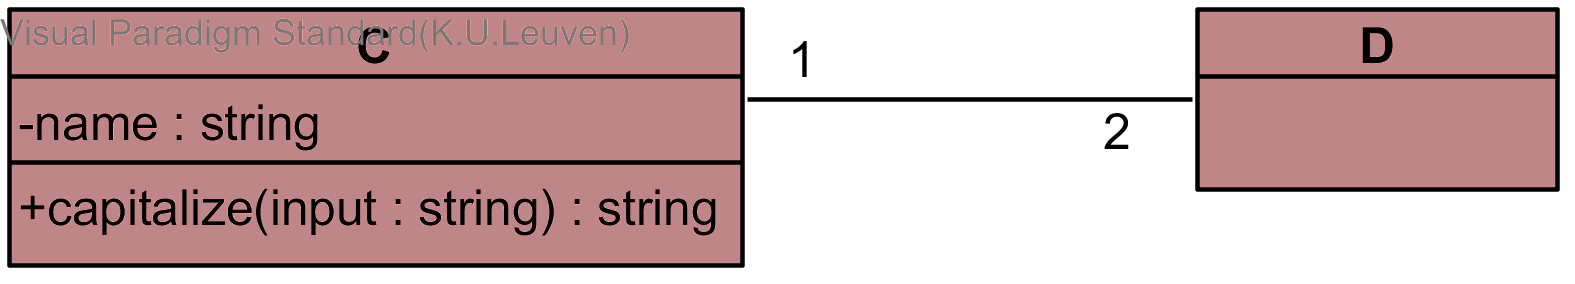
\includegraphics{intro/cd.png}
	\caption{Een voorbeeld van een klassediagram}
\end{figure}

Dit klassediagram drukt uit dat er twee klasses bestaan: \textit{C} en \textit{D}. \textit{C} heeft \'e\'en attribuut, \textit{name}, dat van type \textit{string} is. \textit{D} heeft ook \'e\'en attribuut, \textit{number}, van type \textit{int}. \textit{C} heeft ook \'e\'en operatie \textit{getDNumber} dat \textit{index}, van type \textit{int}, als parameter heeft. \textit{getDNumber(int)} geeft een resultaat terug dat ook van type \textit{int} is. Voorts drukt de lijn tussen \textit{C} en \textit{D} uit dat er een relatie bestaat tussen de twee klasses. Beschouw klasse C. Als we vanuit die klasse de lijn volgen, zien we dat er aan het ander uiteinde staat dat elke \textit{C}-object in relatie moet staan tot exact twee \textit{D}-objecten. Zo ook zien we dat, als we vertrekken vanuit \textit{D}, elk \textit{D}-object in relatie moet staan tot exact \'e\'en \textit{C}-object.

\subsection{Dynamisch domein}

Artefacten in het dynamisch domein bekijken het softwaresysteem vanuit de volgende oogpunten:

\begin{itemize}
	\item Het toestandsautomaatoogpunt: Hieronder vallen toestandsautomaatdiagrammen. Deze diagrammen benoemen toestanden waarin het systeem zich kan bevinden en de mogelijke overgangen tussen de toestanden.
	\item Het activiteitsoogpunt: Hieronder vallen activiteitsdiagrammen. Deze diagrammen beschrijven hoe de besturingsstroom van het systeem kan verlopen tussen activiteiten. Activiteiten zijn processen die bestaan in het systeem.
	\item Het interactieoogpunt: Hieronder vallen sequentiediagrammen en communicatiediagrammen.
	\begin{itemize}
		\item Sequentiediagrammen beschrijven een tijdverloop van een interactie tussen objecten die instanties zijn van klasses gedefinieerd in een klassediagram. Deze diagrammen beschrijven hoe de toestand van \'e\'en of meerdere objecten verandert ten gevolge van een oproep van een methode gedefinieerd voor de klasse waar een bepaald object een instantie van is. Indien de operatie een resultaat heeft, wordt ook getoond hoe het resultaat wordt berekend.
		\item Communicatiediagrammen zijn gelijkaardig aan sequentiediagrammen, maar in plaats van het tijdverloop centraal te stellen tonen ze expliciet hoe de objecten betrokken in een oproep met elkaar in verband staan. 
	\end{itemize}
\end{itemize}

Aangezien sequentiediagrammen het tweede soort diagram zijn dat we beschouwen in deze masterproef, geven we ook daar een klein voorbeeld van. Beschouw volgend sequentiediagram:

\begin{figure}[H]
	\label{fig:sd}
	\centering
	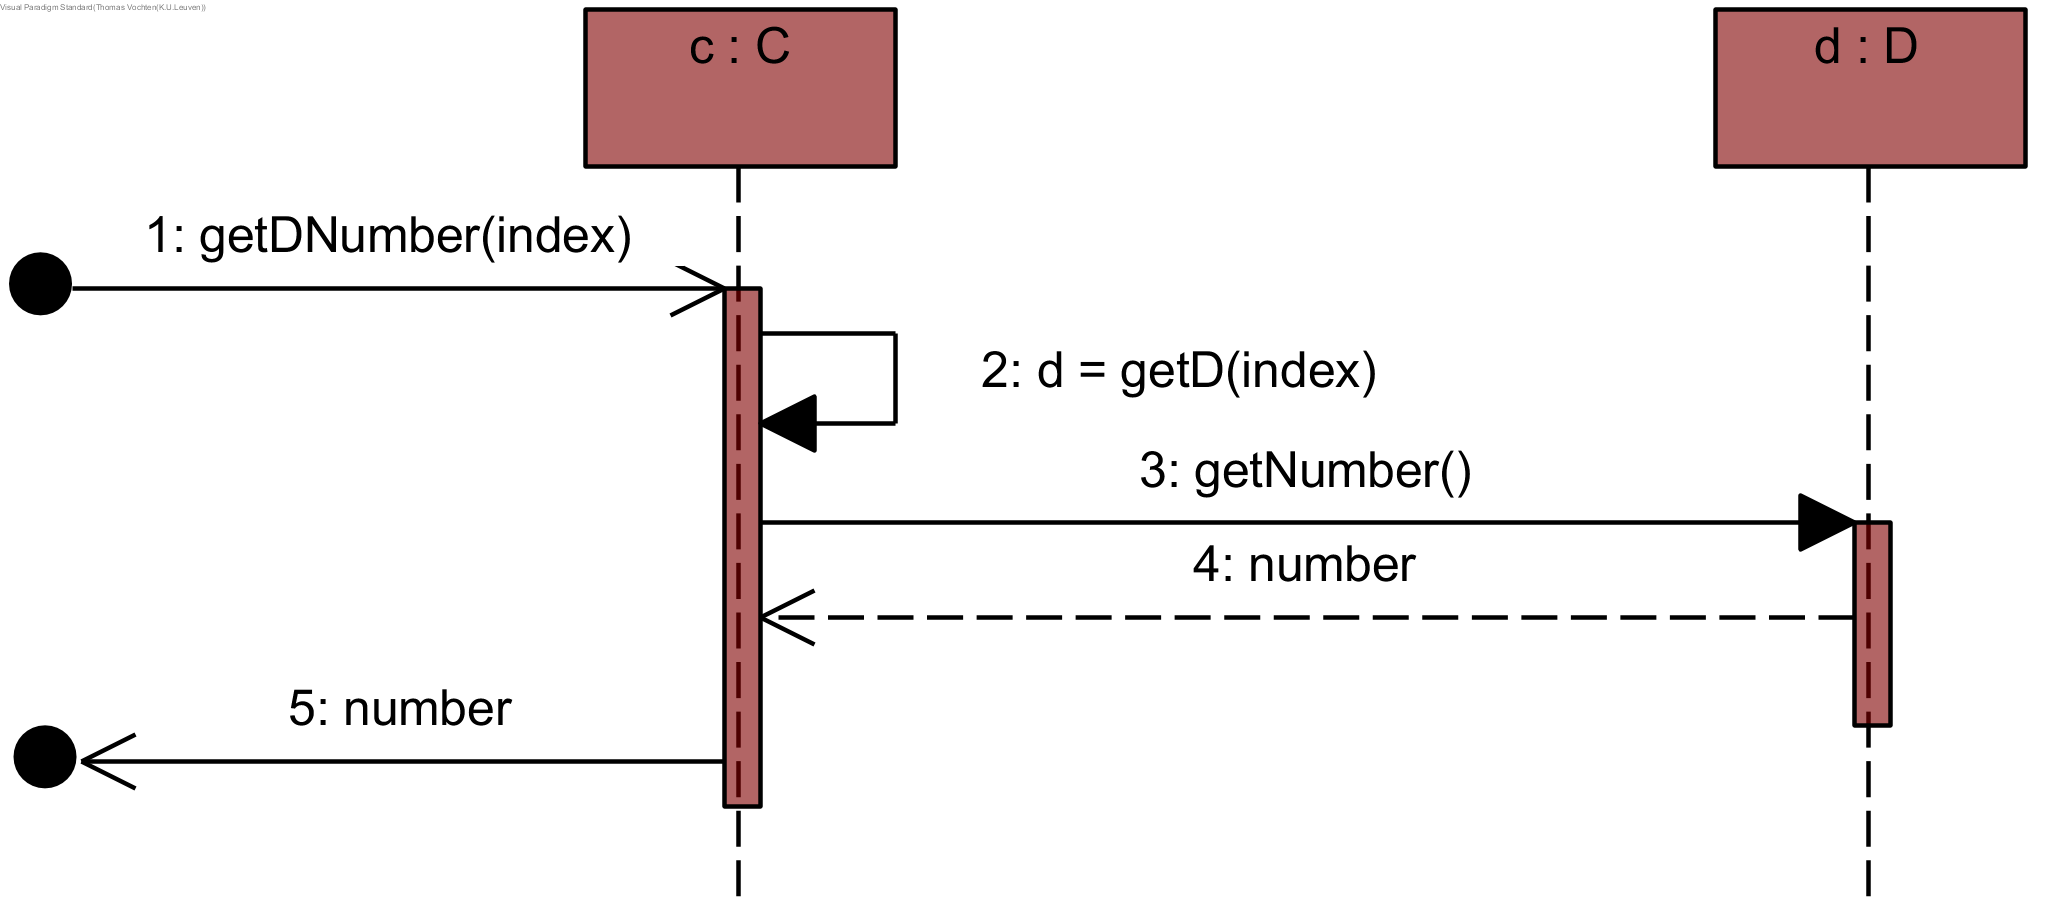
\includegraphics{intro/sd.png}
	\caption{Een voorbeeld van een sequentiediagram}
\end{figure}

Het toont hoe de juiste instantie van \textit{D} wordt opgehaald op basis van invoervariabele \textit{index} en hoe de waarde van het attribuut \textit{number} wordt doorgegeven aan instantie \textit{c}. \textit{c} geeft dan \textit{number} door als uitvoer van het sequentiediagram. Hoofdstuk \ref{sec:gedrag} legt meer in detail uit wat de betekenis is van de elementen die kunnen voorkomen in een sequentiediagram.

\subsection{Fysisch domein}

Artefacten in het fysisch domein bekijken het softwaresysteem vanuit het oogpunt van \textit{deployment}. \textit{Deployment} diagrammen geven weer hoe het systeem fysisch ge\"implementeerd wordt. Deze diagrammen benoemen fysische machines, geven aan welke verbindingen er bestaan tussen die machines en tonen welke concrete softwareartefacten draaien op elke machine.

\subsection{Modelbeheerdomein}

In dit domein beoogt men het beheer van de modellering van het systeem zelf. Tot dit domein behoren de \textit{package} diagrammen. Dit soort diagrammen organiseert de verscheidene soorten modelelementen van het softwaresysteem zoals klasses en \textit{use cases} in \textit{packages}. Een \textit{package} kan ook andere \textit{packages} bevatten. \textit{Package} diagrammen tonen welke \textit{packages} afhankelijk zijn van welke andere \textit{packages}. Zo krijgt men dus een beeld van welke modellen gebruik maken van elementen gedefinieerd in een ander model in hun beschrijving.

\section{Het kennisbanksysteem IDP}\label{sec:intro-idp}

Kennisbanksystemen\cite{1999XKSS} beogen het modelleren van kennis over een probleemdomein op een gestructureerde manier in een kennisbank. Ze bieden inferentiemethodes aan waarmee geredeneerd kan worden op die kennis. Zo kan een kennisbanksysteem nieuwe, meer precieze kennis afleiden. Ze laten ook het oplossen van concrete instanties van een probleem binnen het probleemdomein toe.

In deze masterproef gebruiken we IDP\cite{DeCatBroes2014PLaa}. In IDP zijn kennisbanken opgesteld in FO($\cdot$), een uitbreiding van predicatenlogica.

IDP bouwt verder op eerder werk in het onderzoeksdomein van het logisch programmeren. Het ondersteunt constructies gebaseerd op logisch programmeren, in het bijzonder inductieve definities, maar breekt ook met enkele fundamentele idee\"en uit dat paradigma. Logische theorie\"en opgesteld in FO($\cdot$) zijn geen uitvoerbare programma's---ze zijn beschrijvingen van kennis in het beschouwde probleemdomein. In IDP bestaat de fundamentele oplossingsstrategie voor problemen in een toepassingsdomein uit het specificeren van informatie over het domein in logica. De gebruiker past dan een vorm van inferentie toe om een antwoord te krijgen op concrete vragen geformuleerd in termen van het toepassingsdomein.

Bij het opstellen van logische theorie\"en ondersteunt IDP alle concepten uit de klassieke eerste-orde-predicatenlogica: Constanten, variabelen, predicaten, functies en existenti\"ele en universele kwantoren. IDP ondersteunt ook concepten die eerste-orde-predicantelogica uitbreiden. Concreet gaat het over de volgende vier concepten:

\begin{itemize}
	\item \textbf{Logische types}: Alle variabelen gebruikt in een logische zin hebben een type. Dit betekent ook dat alle argumenten van een predicaat en functie en het resultaat van een functie een type hebben.
	\item \textbf{Aggregaten}: Dit zijn de functies \textit{cardinaliteit}, \textit{som}, \textit{product}, \textit{minimum} en \textit{maximum}. De ontwerper specificeert \'e\'en variabele of een tupel van variabelen. Hij bindt die variabele of tupel dan in een logische zin. Als de ontwerper \'e\'en variabele specificeert, worden alle waarden die voldoen aan de logische zin als argument doorgegeven aan de aggregaatfunctie. Als de ontwerper een tupel specificeert, dan wordt voor elke tupel die voldoet aan de zin het eerste element doorgegeven aan de aggregaatfunctie.
	\item \textbf{Inductieve definities}: Dit is een mechanisme om de interpretatie van een predicaat of functie te defini\"eren analoog aan hoe een concept kan gedefinieerd worden in een recursieve definitie in de wiskunde of in verscheidene domeinen van de wetenschap.
	\item \textbf{Parti\"ele functies}: IDP laat toe om een functie te specificeren als \textit{partieel}. Dit betekent dat niet alle elementen van het domein noodzakelijk worden afgebeeld op een element uit het codomein.
\end{itemize}

De inferentievormen die IDP ondersteunt zijn: Modelexpansie gegeven een deels ingevulde structuur; bepalen of een structuur een model is voor een theorie en/of bepalen of een structuur kan uitgebreid worden tot een model voor de theorie; het vinden van optimale modellen gegeven een aggregate term; propagatie, wat gegeven een structuur en een theorie een preciezere structuur geeft die alle oplossingen behoudt; \textit{query}-inferentie, wat alle objecten die beantwoorden aan een bepaalde \textit{query} ophaalt uit een gegeven structuur; deductie; en \textit{theorem proving} door middel van de functie \textit{entails(theory, theory)}.

De basisblokken van een specificatie in IDP zijn als volgt:

\begin{itemize}
	\item \textbf{Vocabularium}: Hier specificeert de ontwerper de logische types die bestaan in het beschouwd domein en de predicaten en functies over die logische types.
	\item \textbf{Theorie}: Hier schrijft de ontwerper zinnen in FO($\cdot$) die bepalen welke structuren over het beschouwde vocabularium modellen zijn. Indien de ontwerper een inconsistente theorie ontwerpt, zullen er geen modellen zijn.
	\item \textbf{Structuur}: De ontwerper vult hier de logische types gedefinieerd in het vocabularium in. \textit{Constructed types} hebben geen invulling nodig aangezien ze al volledig worden gespecificeerd in het vocabularium. De ontwerper kan ook voor \'e\'en of meerdere predicaten aangeven welke tupels wel of geen lid zijn. Hij kan ook voor \'e\'en of meerdere functies specificeren welke elementen uit het domein afgebeeld worden op welk element uit het codomein.
\end{itemize}

De ontwerper kan meerdere vocabularia, theorie\"en en structuren neerschrijven. Elke theorie en structuur kan wel maar de symbolen van \'e\'en vocabularium gebruiken.

Broes De Cat et al.\cite{DeCatBroes2014PLaa} geven een uitgebreidere inleiding tot IDP.

\section{Probleemstellingen}\label{sec:research-q}

Zoals aangehaald in sectie \ref{sec:situering}, kunnen er inconsistenties of onduidelijkheden sluipen in een klassediagram. Het kan ook dat het gedrag gemodelleerd in een sequentiediagram ingaat tegen bepaalde functionele eisen op het softwaresysteem.

\subsection{Probleemstellingen omtrent klassediagrammen}

We beschouwen twee categorie\"en van gebreken in een klassediagram:

\begin{itemize}
	\item \textbf{Inconsistenties:} Het klassediagram is zo opgebouwd dat geen enkele mogelijke toestand van de software kan beantwoorden aan de voorwaarden die worden opgelegd. Dit betekent dat het stuk van de software dat wordt beschreven in het diagram onmogelijk kan werken.
	\item \textbf{Kwaliteitsgebreken:} Deze gebreken hebben een negatieve impact op de kwaliteit van het softwareontwerp. Zo kunnen ze bijvoorbeeld onduidelijkheden in het ontwerp introduceren of het onderhoud van de software \'e\'enmaal ingezet in productie bemoeilijken.
\end{itemize}

We onderzoeken hoe we klassediagrammen kunnen vertalen naar een voorstelling die ons toelaat om automatisch de consistentie van het diagram te controleren en om bepaalde soorten kwaliteitsgebreken op te sporen.

\subsection{Probleemstellingen omtrent sequentiediagrammen}

We willen het volgende uitvoeren voor sequentiediagrammen:

\begin{itemize}
	\item Het simuleren van het gedrag gemodelleerd in een bepaald stel sequentiediagrammen.
	\item Het verifi\"eren of de uitvoer van een sequentiediagram beantwoordt aan de vereisten opgelegd op de methode die dat sequentiediagram modelleert.
	\item Het verifi\"eren of het gedrag gemodelleerd in een stel sequentiediagrammen overeenkomt met gewenst gedrag in het beoogd softwaresysteem. Een voorbeeld van gewenst gedrag is dat een speler in een schaakspel maar \'e\'en stuk van zijn kleur mag bewegen per beurt.
\end{itemize}

We onderzoeken hoe we sequentiediagrammen kunnen vertalen naar een voorstelling die een uitvoering van het systeem kan simuleren. Met die voorstelling verifi\"eren we ook de uitvoer en het gedrag van sequentiediagrammen.

\section{Verdere verloop van deze tekst}\label{sec:text-structure}

Hoofdstuk \ref{sec:literatuur} geeft een overzicht van literatuur omtrent het gebruik van logica om klassediagrammen en bepaalde soorten dynamische diagrammen voor te stellen.

Hoofdstuk \ref{sec:consistentie} beschrijft hoe we FO($\cdot$) gebruiken om klassediagrammen voor te stellen. We tonen aan dat we consistentie van een klassediagram kunnen verifi\"eren, maar dat er verder onderzoek is vereist om inconsistentie te kunnen controleren.

Hoofdstuk \ref{sec:kwaliteitsgebrek} beschrijft een alternatieve voorstellingswijze die we gebruiken om bepaalde kwaliteitsgebreken op te sporen. We tonen aan dat we de aanwezigheid van losstaande klasses, \textit{many-to-many} associaties en onvoldoende nauw gespecificeerde bovengrenzen op een uiteinde van een associatie kunnen detecteren.

In hoofdstuk \ref{sec:gedrag} beschrijven we hoe sequentiediagrammen voor te stellen in lineaire tijdscalculus\cite{BogaertsBart2014Sdsu}, een methode om in FO($\cdot$) dynamische systemen te modelleren.

In hoofdstuk \ref{sec:evaluatie} evalueren we ons vertalingsproces. We modelleren een spel in een klassediagram en een stel sequentiediagrammen. Die diagrammen gebruiken we enerzijds voor een simulatie van het spel en anderzijds om verificaties van gewenste eigenschappen uit te voeren. Daarbij letten we op rekentijd en geheugengebruik. We tonen aan dat we het spel Nim kunnen modelleren in een klassediagram en een stel sequentiediagrammen en dat we met de theorie opgesteld volgens de regels beschreven in hoofdstukken \ref{sec:consistentie} en \ref{sec:gedrag} het verloop van een spel kunnen simuleren. We nemen waar dat er relatief veel tijd en geheugen nodig is om deze simulaties uit te voeren. Verder tonen we aan dat we kunnen verifi\"eren of de uitvoer van een sequentiediagram voldoet aan bepaalde eisen op de methode gemodelleerd in dat sequentiediagram. Als laatste tonen we aan dat we kunnen controleren of de sequentiediagrammen garanderen dat een spelbeurt altijd verloopt zoals voorgeschreven door de spelregels van Nim.

Hoofdstuk \ref{sec:decl-seq} geeft een aanzet om de ontwerptaal beschikbaar voor sequentiediagrammen uit te breiden met declaratieve constructies. Het doel is om ervoor te zorgen dat er significant minder berichten nodig zijn in een sequentiediagram om het gedrag van een methode te specificeren. We modelleren Nim opnieuw met deze constructies en tonen aan dat er significant minder rekentijd en geheugen nodig is om het gedrag in het bekomen sequentiediagram te simuleren.

Hoofdstuk \ref{sec:conclusie} geeft een besluit en geeft een aanzet tot verder onderzoek.
\section{Controleren van consistentie}\label{sec:consistentie}
In dit hoofdstuk treden we meer in detail over hoe we de consistentie van een diagram willen controleren. Daarvoor willen we een specifieke vorm van logische theorie automatisch laten genereren. In deze theorie\"en staan \textbf{objecten} centraal. Deze objecten zijn instanties van een klasse die voorkomt in het beschouwde diagram, hebben exact de attributen en operaties van die klasse en maken deel uit van exact die relaties die het diagram voorschrijft voor die klasse. Aan de hand van volgend voorbeeld zullen we illustreren welke regels we gebruiken om zulk een theorie op te bouwen:

\begin{figure}[H]
	\label{fig:diagram-voorbeeld}
	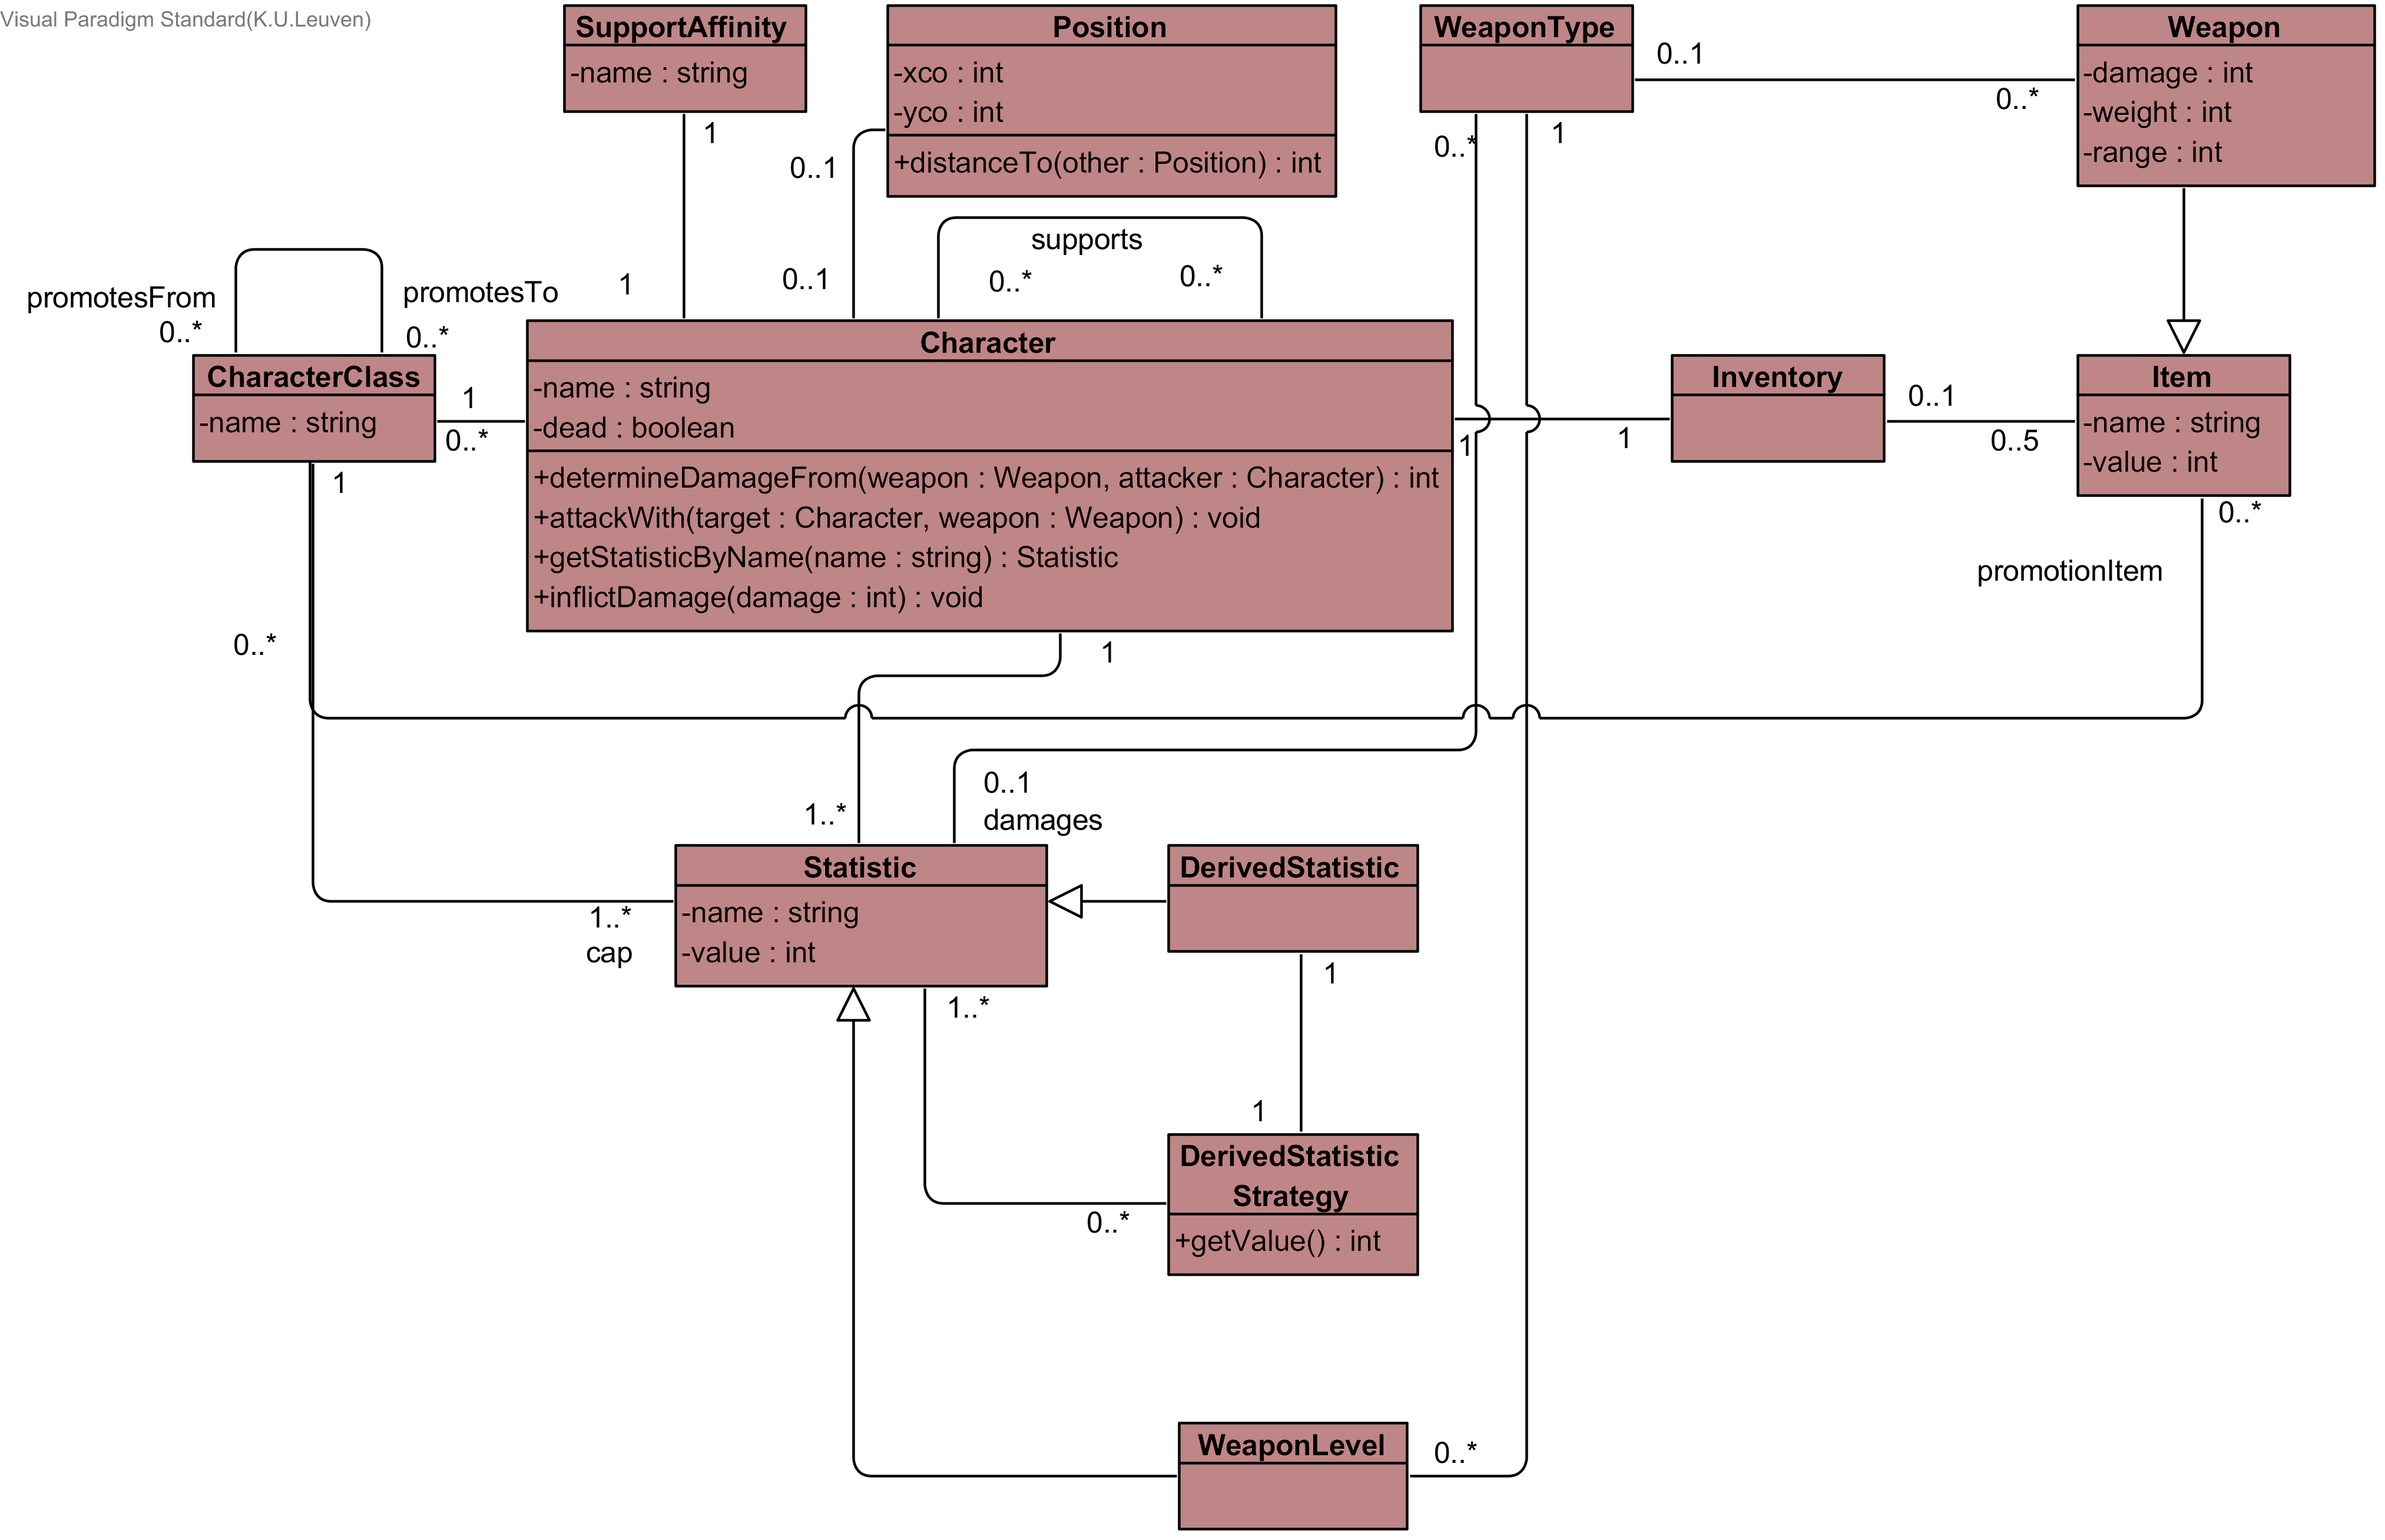
\includegraphics[width=0.95\textwidth]{chap-consistentie/diagram-voorbeeld.png}
	\caption{Leidend voorbeeld van een klassediagram}
\end{figure}

Meer bepaald willen we uitdrukken welke \textbf{klasses} er bestaan in het diagram waarvan een object een instantie kan zijn, welke \textbf{attributen} en \textbf{operaties} elke klasse bevat, welke \textbf{associaties} er bestaan tussen de verscheidene klasses en welke \textbf{klassehi\"erarchie\"en} er bestaan.

\subsection{Logisch type \textit{Object}}
Zoals gezegd staan in deze theori\"en objecten centraal, dus is het vanzelfsprekend om een logisch type \textit{Object} te voorzien. Dit logisch type bevat dus softwareobjecten.

\subsection{Logisch type \textit{ClassObject} en predicaat \textit{StaticClass$\backslash2$}}
Dit logisch type bevat exact de klasses die worden weergegeven in het diagram --- niet meer en niet minder. \textit{Character}, \textit{Inventory}, \textit{Item} enz. zijn dus \textit{ClassObject}s.
We drukken uit dat een \textit{Object} een instantie is van een bepaald \textit{ClassObject} door middel van het predicaat \textit{StaticClass$\backslash2$}. \textit{StaticClass(o1,Character)} zegt dus uit dat het object \textit{o1} een instantie is van klasse \textit{Character}.

\subsection{Voorstellen van attributen}
Voor elk attribuut voegen we een binair predicaat toe waarvan de naam beantwoordt aan het patroon: \textit{Klassenaamattribuutnaam}. Voor klasse \textit{Character} en attribuut \textit{name} resulteert dit dus in het predicaat \textit{Charactername$\backslash2$}. Het eerste argument van dit predicaat is een \textit{Object}. Het type van het tweede argument hangt af van wat er in het diagram staat: Als het een primitief type is zoals \textit{string} of \textit{int}, zal dat ook het type zijn van het tweede predicaat; in het andere geval is het type van het tweede argument ook \textit{Object}.
De signatuur van \textit{Charactername$\backslash2$} is daarom \textit{Charactername(Object, string)}.
Voor elk attribuut worden ook een aantal andere regels afgeleid:

\begin{itemize}
	\item Als het tweede argument van het attribuutpredicaat \textit{Object} is, wordt er een regel toegevoegd van de vorm:
	
	\begin{align*}
	\forall{o1}[Object]\forall{o2}[Object](Klassenaamattribuutnaam(o1,o2) \Rightarrow \\ StaticClass(classObj,o1) \land StaticClass(attrClassObj,o2))
	\end{align*}
	
	waarbij \textit{classObj} het logisch object van type \textit{ClassObject} dat het attribuut bevat en \textit{attrClassObj} het logisch object van type \textit{ClassObject} dat dient als mogelijke waarde van dit attribuut. Deze regel verzekert dat de attribuuthouder en de attribuutwaarde van de juiste klasse zijn. In dit diagram komt dit geval nergens voor en wordt deze regel dus niet toegepast.
	
	\item Als het tweede argument van het attribuutpredicaat van een primitief type is, wordt een regel toegevoegd van de vorm:
	
	\begin{align*}
	\forall{o}[Object]\forall{x}[primitiveType](Klassenaamattribuutnaam(o,x) \Rightarrow \\ StaticClass(classObj,o))
	\end{align*}
	
	waarbij primitiveType het type van de attribuutwaarde. De signatuur van het predicaat verzekert dat de attribuutwaarde van het juiste type is, dus moet dit niet explicit worden neergeschreven. Deze regel zorgt ervoor dat de volgende zin wordt toegevoegd aan de theorie:
	
	\begin{align*}
	\forall{o}[Object]\forall{x}[primitiveType](Charactername(o,x) \Rightarrow \\ StaticClass(Character,o))
	\end{align*}
	
	\item De multipliciteit van het attribuut wordt ook in rekening gebracht. Zij \textit{lowerBound} de ondergrens en \textit{upperBound} de bovengrens. Dan is de meest algemene vorm van deze regel als volgt:
	
	\begin{align*}
	\forall{o1}[Object](StaticClass(classObj,o1) \Rightarrow lowerBound \geq \\ \#\{o2: Klasseattribuutnaam(o1,o2)\} \geq upperBound
	\end{align*}
	
	waarbij \textit{lowerBound} wordt weggelaten als deze $0$ is en \textit{upperBound} wordt weggelaten als deze $*$ is. Indien beide van deze voorwaarden gelden, wordt er geen regel afgeleid betreffende de multipliciteit van het attribuut. Als $lowerBound = upperBound$, wordt deze regel in de plaats:
	
	\begin{align*}
	\forall{o1}[Object](StaticClass(classObj,o1) \Rightarrow \\ \exists_{=upperBound}{o2}(Klassenaamattribuutnaam(o1,o2))
	\end{align*}
	
	Voor \textit{Charactername$\backslash2$} wordt daarom afgeleid:
	
	\begin{align*}
	\forall{o}[Object](StaticClass(Character,o) \Rightarrow \exists_{=1}{x}(Charactername(o,x))
	\end{align*}
\end{itemize}

\subsection{Voorstellen van operaties}
Voor elke operatie voegen we een predicaat toe dat beantwoordt aan volgend patroon: \textit{Klassenaamoperatienaam$\backslash(m+2)$}, waarbij $m$ het aantal argumenten dat als invoer wordt meegegeven aan de operatie. De signatuur ziet eruit als \\ \textit{$Klasseoperatienaam(o,p_1,\ldots,p_m,r)$}, waarbij \textit{o} het object van logisch type \textit{Object} waarop de operatie wordt opgeroepen, \textit{$p_1$} \ldots \textit{$p_m$} de argumenten en \textit{r} het resultaat van de oproep van de operatie op het object \textit{o} met de gegeven argumenten. Indien er geen argumenten zijn, ziet de signatuur eruit als \textit{Klassenaamoperatienaam(o,r)}. Voor \textit{determineDamageWeaponFrom(Weapon)} van \textit{Character} wordt dit dus \textit{CharacterdetermineDamageFrom(Object,Object,int)}.

Voor elke operatie worden de volgende regels afgeleid:

\begin{itemize}
	\item Het object waarop de operatie wordt opgeroepen (zijnde \textit{o}), de parameters (zijnde \textit{$p_1 \ldots p_m$}) en het resultaat van de oproep (zijnde \text{r}) moeten allemaal van de juiste klasse zijn. Daarom wordt een regel toegevoegd van de vorm:
	
	\begin{align*}
	&\forall{o}[Object]\forall{p_1}[Object]\ldots\forall{p_m}[Object]\forall{r}[Object]
	\\
	&(Klassenaamoperatienaam(o,p_1,\ldots,p_m,r) \Rightarrow
	\\ 
	&StaticClass(classObj,o) \land StaticClass(p_{1}ClassObj,p_1) \land \ldots \land
	\\
	&StaticClass(p_{m}ClassObj,p_m) \land StaticClass(resultClassObj,r))
	\end{align*}
	
	Voor elke \textit{p} waarvoor geldt dat het van een primitief type is wordt de corresponderende \textit{StaticClass($p_l,p_{l}ClassObj$)} (met $1 \leq l \leq m$) weggelaten; hetzelfde geldt voor \textit{r}.
	De invulling voor \textit{CharacterdetermineDamageFrom(o,p1,r)} wordt dus:
	
	\begin{align*}
	\forall{o}[Object]\forall{p_1}[Object](CharacterdetermineDamageFrom(o,p_1,r) \Rightarrow \\
	StaticClass(Character,o) \land StaticClass(Weapon,p_1))
	\end{align*}
	
	\item Voor elke combinatie van Object waar de operatie wordt opgeroepen en invoerparameters moet gelden dat er exact \'e\'en resultaat is:
	
	\begin{align*}
	&\forall{o}[Object]\forall{p_1}[Object]\ldots\forall{p_m}[Object]
	\\
	&(StaticClass(classObj,o) \land StaticClass(p_{1}ClassObj,p_1) \land \ldots \land
	\\
	&StaticClass(p_m,p_{m}ClassObj) \Rightarrow
	\\
	&\exists!{r}[Object](Klassenaamoperatienaam(o,p_1,\ldots,p_m,r)))
	\end{align*}
	
	Opnieuw geldt dat voor primitieve types de bijhorende conjuncten weggelaten worden. De invulling voor \textit{CharacterdetermineDamageFrom(Object,Object,int)} wordt:
	
	\begin{align*}
	&\forall{o}[Object]\forall{p_1}[Object](StaticClass(Character,o) \land
	\\
	&StaticClass(Weapon,p_1) \Rightarrow \exists!{r}(CharacterdetermineDamageFrom(o,p1,r))
	\end{align*}
\end{itemize}

\subsection{Voorstellen van associaties}
Voor elke associatie voegen we een predicaat toe dat beantwoordt aan volgend patroon: \textit{$ClassOneand\ldots{}andClassM\backslash{m}$}, waarbij \textit{m} de ariteit van de associatie. Voor de associatie tussen \textit{Inventory} en \textit{Item} wordt dit dus \textit{InventoryandItem(Object,Object)}. We leiden regels van de volgende vormen af voor elke associatie:

\begin{itemize}
	\item De deelnemende Objects moeten allemaal van de juiste klasse zijn. Daarom wordt een regel toegevoegd van de vorm:
	
	\begin{align*}
	\forall{o_1}[Object]\ldots\forall{o_m}[Object](ClassOne\ldots{}andClassM(o_1,\ldots,o_m) \\ \Rightarrow StaticClass(o_{1}ClassObj,o_1) \land \ldots \land StaticClass(o_{m}ClassObj,o_m))
	\end{align*}
	
	Voor \textit{InventoryandItem(Object,Object)} wordt dit:
	
	\begin{align*}
	\forall{o_1}[Object]\forall{o_2}[Object](InventoryandItem(o1,o2) \Rightarrow \\ StaticClass(Inventory,o1) \land StaticClass(Item,o2))
	\end{align*}
	
	\item De multipliciteit voor elke rol moet worden uitgedrukt. Voor alle $o_l$ waarvoor $1 \leq l \leq m$ wordt een regel toegevoegd van de volgende vorm:\\
	Zij $lowerBound_l$ de ondergrens en $upperBound_l$ de bovengrens:
	\begin{align*}
	&\forall{c_1}[Object]\ldots\forall{c_m}[Object](StaticClass(c_{1}ClassObj,c_1) \land \ldots \land
	\\
	&StaticClass(c_{m}ClassObj,c_m) \Rightarrow lowerBound_l \leq
	\\
	&\#{o_l: ClassOneand\ldots{}ClassM(c_1,\ldots,o_1,\ldots,c_m)} \leq upperBound_l)
	\end{align*}
	
	waarbij de \textit{c} met index \textit{l} overgeslagen wordt. Indien de ondergrens gelijk is aan $0$ of de bovengrens gelijk is aan $*$ worden dezen weggelaten. Als beide voorwaarden gelden, wordt voor deze \textit{l} geen regel afgeleid. Indien $lowerBound_l = upperBound_l$ wordt in de plaats afgeleid:
	
	\begin{align*}
	&\forall{c_1}[Object]\ldots\forall{c_m}[Object](StaticClass(c_{1}ClassObj,c_1) \land \ldots \land
	\\
	&StaticClass(c_{m}ClassObj,c_m) \Rightarrow \\ &\exists_{=upperbound_l}o_l(ClassOneand\ldots{}andClassM(c_1,\ldots,o_l,\ldots,c_m)))
	\end{align*}
	
	Voor \textit{InventoryandItem$\backslash{}m$} worden de volgende regels afgeleid:
		\begin{align*}
		\forall{o_2}[Object](StaticClass(Item,o_2) \Rightarrow \\ \#{o_1: InventoryandItem(o_1,o_2)} \leq 1)
		\end{align*} 
		
		\begin{align*}
		\forall{o_1}[Object](StaticClass(Inventory,o_1) \Rightarrow \\ \#{o_2: InventoryandItem(o_1,o_2)} \leq 5)
		\end{align*}
\end{itemize}

\subsection{Voorstellen van klassehi\"erarchi\"een}
Stel dat voor een object \textit{o} van logisch type \textit{Object} gegeven is dat \textit{StaticClass(oClassObject,o)}. Ons doel is dat \textit{StaticClass(superClassObject,o)} geldt voor alle objecten van logisch type \textit{ClassObject} die volgens het diagram superklasses zijn van \textit{oClassObject} --- niet meer en niet minder. Daartoe introduceren we het predikaat \textit{IsDirectSupertypeOf(ClassObject,ClassObject)} dat ingevuld wordt door alle directe subklasseringen van het diagram en het predikaat \textit{IsSupertypeOf(ClassObject,ClassObject)}, hetgeen de transitieve sluiting is van \textit{IsDirectSupertypeOf}. Om zowel de invulling van \textit{IsDirectSupertypeOf$\backslash2$} te doen als de transitieve sluiting te berekenen maken we gebruik van \textbf{inductieve definities} voor twee redenen:

\begin{enumerate}
	\item In predikatenlogica is het onmogelijk om op een universeel geldige manier de transitieve sluiting uit te drukken.
	\item Als men in een inductieve definitie een lijst feiten opsomt, drukt men tegelijk ook uit dat exact die feiten waar zijn --- niet meer of niet minder.
\end{enumerate}

In \'e\'en definitie lijsten we dus de feiten die we kunnen aflezen van het diagram op:

\begin{align*}
\{
	IsDirectSupertypeOf(Statistic,Weaponlevel) \leftarrow \\
	IsDirectSupertypeOf(Statistic,DerivedStatistic) \leftarrow \\
	IsDirectSupertypeOf(Item,Weapon) \leftarrow \\
\}
\end{align*}

In een andere definitie drukken we de transitieve sluiting uit en gebruiken we die ook meteen om het gewenste resultaat voor \textit{StaticClass$\backslash2$} uit te komen:

\begin{align*}
\{
	&\forall{x}[ClassObject]\forall{y}[ClassObject](IsSupertypeOf(x,y) \leftarrow \\ &IsDirectSupertypeOf(x,y)) \\
	&\forall{x}[ClassObject]\forall{y}[ClassObject](IsSupertypeOf(y,x) \leftarrow \\
	&\exists{z}(IsSupertypeOf(y,z) \land IsSupertypeOf(z,x)))
	\\
	\\
	&\forall{x}[ClassObject]\forall{o}[Object](StaticClass(x,o) \leftarrow RuntimeClass(x,o)) \\
	&\forall{x}[ClassObject]\forall{y}[ClassObject]\forall{o}[Object](StaticClass(y,o) \leftarrow \\ &RuntimeClass(x,o) \land IsSupertypeOf(y,x))
\}
\end{align*}

waarbij \textit{RuntimeClass(ClassObject,Object)} een predikaat is dat uitdrukt wat de uniek dynamisch bepaalde klasse is van een \textit{Object} (de veronderstelling is dat in een geldige toestand van een programma in uitvoering ieder object exact \'e\'en \textit{runtime} klasse heeft).
\\
In hoofdstuk \ref{sec:rol-idp} wordt de logische theorie die automatisch gegenereerd werd volgens de regels opgelijst in dit hoofdstuk weergegeven en wordt ook uitgelegd hoe die theorie wordt gebruikt om de consistentie van het diagram te controleren.
\chapter{Controleren op kwaliteitsgebreken}\label{sec:kwaliteitsgebrek}
Waar in hoofdstuk \ref{sec:consistentie} \textit{Object}s centraal stonden, doen we daar hier afstand van: we abstraheren \textit{Object}s weg en concentreren ons in de plaats op \textit{ClassObject}s. We gebruiken het diagram in figuur \ref{fig:diagram-voorbeeld} weer als begeleidend voorbeeld. In de volgende subsecties overlopen we hoe we de theorie die we gebruiken voor dit probleem opbouwen.

\subsection{Gebruikte logische types en predikaten}
We bewaren het logisch type \textit{ClassObject} en het predikaat \textit{IsSupertypeOf(ClassObject,\\ClassObject)} exact zoals ze zijn in hoofdstuk \ref{sec:consistentie} (en berekenen de transitieve sluiting horende bij \textit{IsSupertypeOf$\backslash2$} op dezelfde manier) en gebruiken daar bijkomend volgende predikaten:

\begin{itemize}
	\item \textbf{\textit{BiAssoc(ClassObject,ClassObject)}}: drukt uit dat er een binaire associatie bestaat tussen de twee klasses.
	\item \textbf{\textit{BiAssocLow(ClassObject,ClassObject,ClassObject,nat)}}: voor \textit{BiAssocLow(x,y,x,n1)} geldt dat voor de binaire associatie tussen klasse \textit{x} en klasse \textit{y} de ondergrens voor de multipliciteit aan de \textit{x}-kant gelijk is aan \textit{n1}; een gelijkaardige interpretatie geldt voor \textit{BiAssocLow(x,y,y,n2)}.
	\item \textbf{\textit{BiAssocHigh(ClassObject,ClassObject,ClassObject,nat)}}: gelijkaardig aan \textit{BiAssocLow$\backslash4$}, maar dan voor de bovengrens van de multipliciteit.
\end{itemize}

Deze predikaten worden ingevuld met een lijst van feiten die af te lezen zijn van het diagram. In hoofdstuk \ref{sec:rol-idp} wordt de logische theorie die het resultaat is van dit proces weergegeven.

\subsection{Kwaliteitsgebreken detecteren}
Er zijn drie kwaliteitsgebreken waarnaar wordt gezocht in de resulterende theorie:

\begin{itemize}
	\item \textbf{Many-to-many associaties}: Dit zijn associaties waar dat de bovengrens van de multipliciteiten aan beide kanten gelijk is aan $*$. Het voorkomen van een many-to-many associatie is doorgaans een teken dat er een klasse ontbreekt in het ontwerp. Het is dus van groot belang dat dit wordt opgespoord en opgelost.
	
	\item \textbf{Losstaande klasse}: Concreet is een losstaande klasse een klasse die geen associatie heeft met een andere klasse in het ontwerp. Zulk een klasse is nutteloos en moet ofwel verbonden worden met een andere klasse of verwijderd worden.
	
	\item \textbf{Overbodige associaties in een klassehi\"erarchie}: Beschouw figuur \ref{fig:hierarchie}. Daar is te zien dat de grenzen van de multipliciteiten in de associatie \textit{Alice}---\textit{Charlie} strengere voorwaarden opleggen dan die van de associatie \textit{Bob}---\textit{David}, en dat daarom de associatie \textit{Bob}---\textit{David} overbodig is. Om de verstaanbaarheid van het diagram te verbeteren, wordt die associatie best verwijderd.
\end{itemize}

We defini\"eren deze respectievelijke gebreken in de logische theorie door middel van de volgende logische zinnen:

\begin{align*}
	\forall{x}[ClassObject]\forall{y}[ClassObject](ManyToMany(x,y) \Leftrightarrow BiAssoc(x,y) \land \\ \lnot\exists{z}[nat](BiAssocHigh(x,y,x,z)) \land \lnot\exists{z}[nat](BiAssocHigh(x,y,y,z)))
\end{align*}

\begin{align*}
	\forall{x}[ClassObject](LooseClass(x) \Leftrightarrow \lnot(\exists{y}[ClassObject](BiAssoc(x,y)) \\ \lor \exists{s}[ClassObject]\exists{y}[ClassObject](IsSupertypeOf(s,y) \land BiAssoc(s,x)))
\end{align*}

\todo{oplossing vinden voor de derde: gewoon verwijzen naar IDP-bestand?}

\begin{figure}
	\label{fig:hierarchie}
	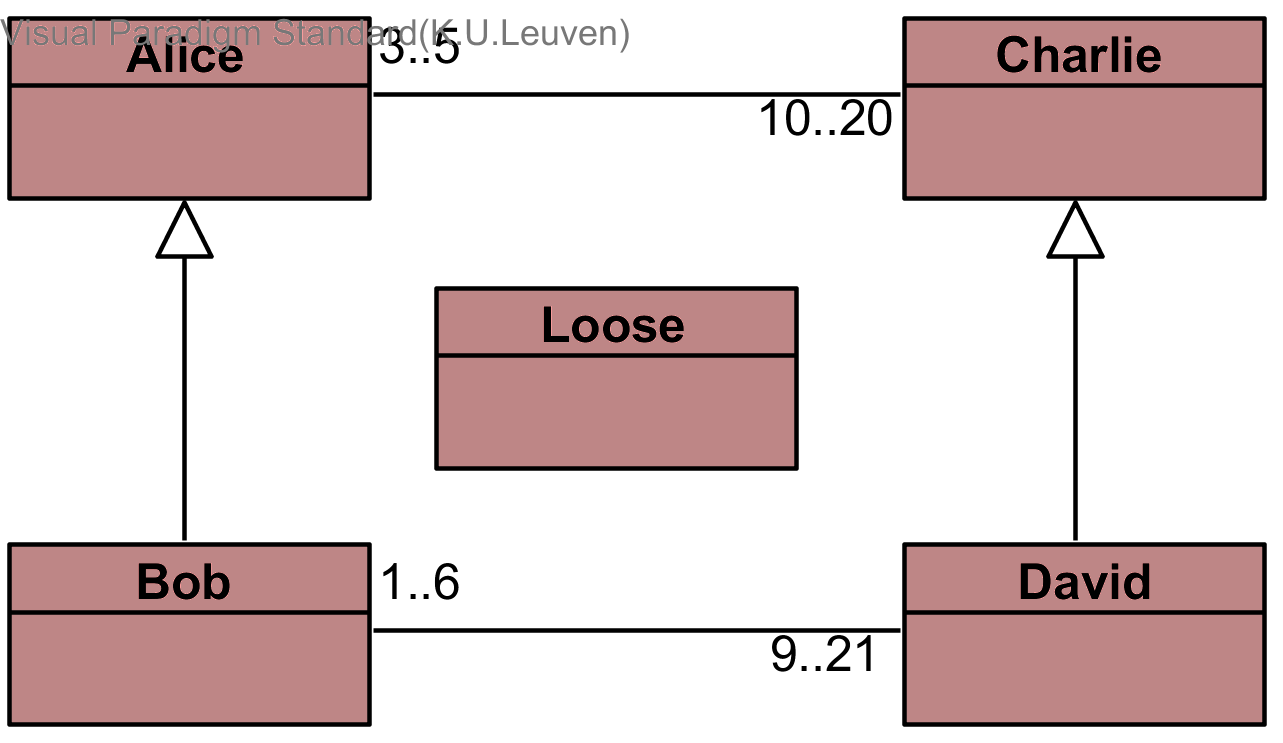
\includegraphics{chap-kwaliteitsgebrek/hierarchy.png}
	\caption{Voorbeeld van meer permissieve multipliciteiten in een klassehi\"erarchie en van een losstaande klasse (zijnde \textit{Loose})}
\end{figure}

Deze regels worden meteen toegevoegd aan de theorie die wordt gegenereerd zoals uitgelijnd eerder in dit hoofdstuk. In hoofdstuk \ref{sec:rol-idp} wordt uitgelegd hoe deze theorie wordt gebruik om kwaliteitsgebreken te vinden.
\chapter{Het kennisbanksysteem IDP}\label{sec:rol-idp}
\section{Korte inleiding in IDP}
IDP is een kennisbanksysteem\cite{DeCatBroes2014PLaa}. Deze kennisbanken zijn opgesteld in FO($\cdot$), een uitbreiding van predicatenlogica. De basisblokken van een specificatie in IDP zijn als volgt:

\begin{itemize}
	\item \textbf{Vocabularium}: Hier specificeert de ontwerper de logische types die bestaan in het beschouwd domein en de predicaten en functies over die logische types.
	\item \textbf{Theorie}: Hier schrijft de ontwerper zinnen in FO($\cdot$) die bepalen welke structuren over het beschouwde vocabularium modellen zijn. Indien de ontwerper een inconsistente theorie ontwerpt, zullen er geen modellen zijn.
	\item \textbf{Structuur}: De ontwerper vult hier de logische types gedefinieerd in het vocabularium in. \textit{Constructed types} hebben geen invulling nodig aangezien ze al volledig worden gespecificeerd in het vocabularium. De ontwerper kan ook voor \'e\'en of meerdere predicaten aangeven welke tupels wel of geen lid zijn. Hij kan ook voor \'e\'en of meerdere functies specificeren welke elementen uit het domein afgebeeld worden op welk element uit het codomein.
\end{itemize}

De ontwerper kan meerdere vocabularia, theorie\"en en structuren neerschrijven. Elke theorie en structuur kan wel maar de symbolen van \'e\'en vocabularium gebruiken.

IDP gebruikt zijn eigen symbolen voor universele kwantoren, existenti\"ele kwantoren en logische connectieven. \cite{DeCatBroes2014PLaa} bevat een uitgebreidere inleiding tot IDP.

\section{Gebruik van modeluitbreiding}
Gegeven een structuur over een bepaald vocabularium kan de gebruiker de opdracht geven aan IDP om een uitbreiding te vinden van deze structuur die ervoor zorgt de structuur een model is van een gegeven theorie. Dit is een vorm van inferentie die men \textbf{modeluitbreiding} noemt. Het kan echter het geval zijn dat IDP antwoordt dat zulk een uitbreiding niet bestaat of dat de uitvoering nooit eindigt.


\subsection{Controleren van consistentie}
In bijlage \ref{app:consistentie} staat de logische theorie die werd gegenereerd volgens de regels uitgelijnd in hoofdstuk \ref{sec:consistentie}. Als men dit geeft als invoer aan IDP, is het besluit dat er een model bestaat voor de theorie en dat het diagram inderdaad consistent is.

\subsection{Detecteren van kwaliteitsgebreken}
In bijlage \ref{app:kwaliteitsgebrek} staat de logische theorie die werd gegenereerd uit een combinatie van de diagrammen uit figuren \ref{fig:diagram-voorbeeld} en \ref{fig:hierarchie} volgens de regels uitgelijnd in hoofdstuk \ref{sec:kwaliteitsgebrek}. IDP vindt alle many-to-many associaties, besluit dat \textit{Loose} een losstaande klasse is en dat de associatie \textit{Bob}---\textit{David} overbodig is door de samenloop van de klassehi\"erarchie en de opgelegde multipliciteiten.

\backmatter

\end{document}